
  De acordo com Leffingwell (\citeyear{leffingwell11}), o \textit{Roadmap} consiste numa série de \textit{releases} planejadas em datas, onde cada
  uma delas possui um tema e uma lista de \textit{features} priorizadas.
  
   \begin{figure}[!htbp]
    \centering
    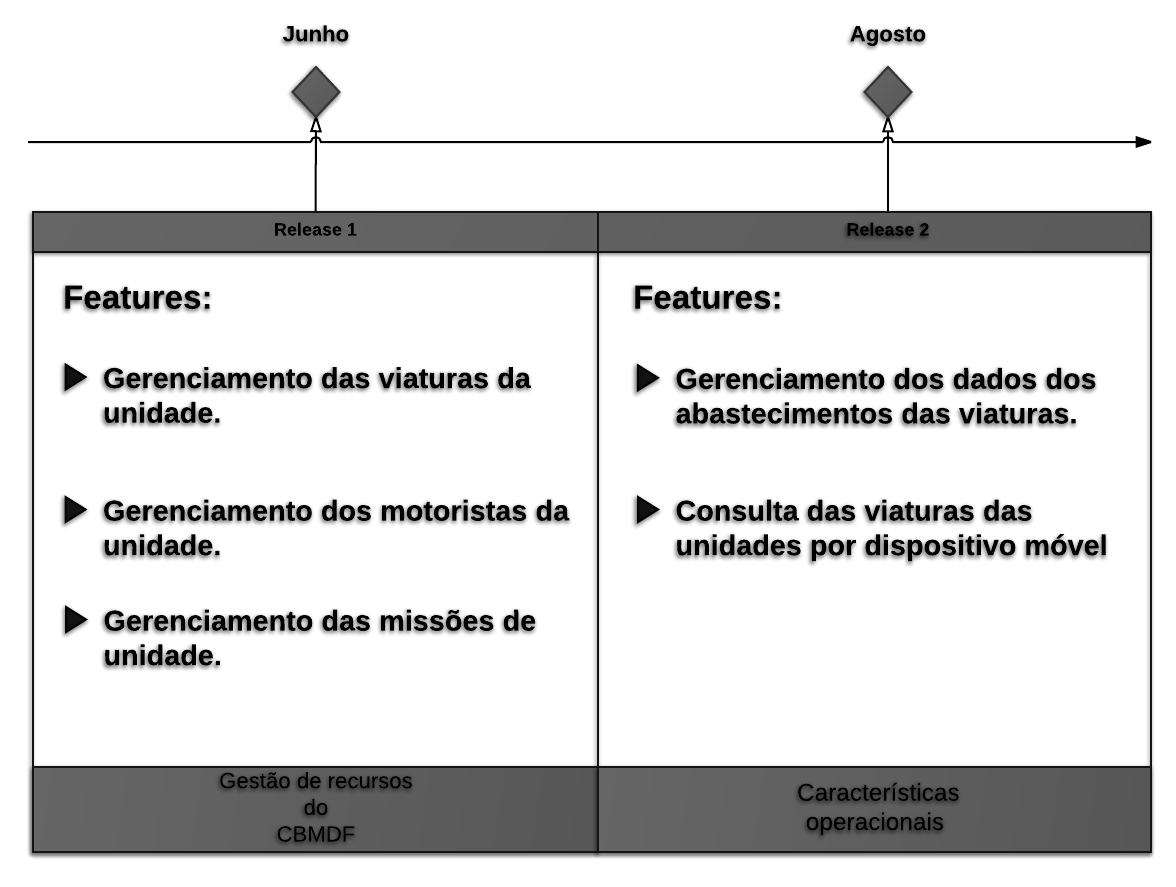
\includegraphics[scale=0.4, angle=0]{figuras/roadmap}
    \caption[\textit{Roadmap} do projeto.]{\textit{Roadmap} do projeto.}
    \label{fig:roadmap}
  \end{figure}
  
  Como ilustrado da Figura \ref{fig:roadmap} acima, o \textit{Roadmap} do projeto é composto por duas \textit{releases} com seus
  respectivos temas e datas. As \textit{features} foram alocadas e priorizadas, nas \textit{releases} a partir dos critérios: 
  
  \begin{itemize}
   \item Dependência funcional entre os requisitos;
    \subitem As \textit{features} estão alocadas em ordem de dependência funcional (de cima para baixo), bem como entre as
    \textit{releases} (da esquerda para direita).
    
   \item Importância relativa das mesmas para o cliente.
    \subitem As \textit{features} alocadas na \textit{release} 1 possuem maior importância e agregam maior valor ao cliente.
  \end{itemize}
